\documentclass[a4paper,12pt]{article} % This defines the style of your paper

\usepackage[top = 2.5cm, bottom = 2.5cm, left = 2.5cm, right = 2.5cm]{geometry} 

\usepackage[T2A]{fontenc}
\usepackage[utf8]{inputenc}
\usepackage[russian]{babel}

\usepackage{multirow} 
\usepackage{booktabs} 

\usepackage{graphicx} 

\usepackage{setspace}
\setlength{\parindent}{0in}

\usepackage{float}

\usepackage{amsmath}

\usepackage{fancyhdr}

\usepackage{pgfplots}
\pgfplotsset{compat=1.9}

\pagestyle{fancy} 

\fancyhf{} 

\lhead{\footnotesize Расчетное задание №17}

\rhead{\footnotesize Николаев Юрий} 

\cfoot{\footnotesize \thepage} 

\begin{document}

\thispagestyle{empty} 

\begin{tabular}{p{15.5cm}} 
НИУ МЭИ \\ А-13а-19  \\ Вариант 13 \\ Николаев Юрий\\
\hline 
\\
\end{tabular} 

\vspace*{0.3cm}

\begin{center} 
	{\Large \bf Расчетное задание №17} 
	\vspace{2mm}
\end{center}  

\vspace{0.4cm}


\section{Задание}
Функция $y = y(x)$ задана таблицей своих значений. Построить параболический сплайн дефекта 1 для функции $y = y(x)$, если известно также дополнительное условие. На одном чертеже построить график сплайна и указать исходные точки 

$(x_i, y_i), i = 0, ..., 3$.

\vspace{0.4cm}

УКАЗАНИЕ. Для упрощения вычислений записать многочлен на отрезке $[x_{i - 1}, x_i]$ в виде $P_i(x) = a_{i, 0} + a_{i, 1}(x - x_{i - 1}) + a_{i, 2}(x - x_{i - 1})(x - x_i)$.

\begin{center}
\begin{tabular}{| c | c | c | c | c |}
\hline
    x & 0 & 1 & 2 & 3 \\ \hline
    y & 6 & -10 & -29 & -58 \\
\hline
\end{tabular}

\vspace{0.4cm}

Дополнительное условие: $S''(2 - 0) = S''(2 + 0)$
\end{center}

\section{Решение}

\begin{enumerate}

\item Сплайн $S_2$ будет представлять систему систему из трех полиномов 3-й степени:
\begin{equation*}
    S_2(x) =
    \begin{cases}
        P_{1, 1} = a_{1, 0} + a_{1, 1}x + a_{1, 2}x^2, x \in [0, 1]\\
        P_{1, 2} = a_{2, 0} + a_{2, 1}x + a_{2, 2}x^2, x \in [1, 2]\\
        P_{1, 3} = a_{3, 0} + a_{3, 1}x + a_{3, 2}x^2, x \in [2, 3]
    \end{cases}
\end{equation*}

Сплайн удовлетворяет условиям:

$S_2(x_i) = y_i$, $i = 0, ..., 3$ - условие интерполяции

$S_2(x_{i - 1}) = y_{i - 1}$, $i = 1, ..., 3$ - условие интерполяции

$P'_{1, 1}(1) = P'_{1, 2}(1)$ - условие непрерывности первой производной

$P'_{1, 2}(2) = P'_{1, 3}(2)$ - условие непрерывности первой производной

$P''_{1, 2}(2) = P''_{1, 3}(2)$ - дополнительное условие

\newpage

\item Получили 9 уравнений и 9 неизвестных, решим систему и найдем нужные коэффициенты:
\begin{equation*}
    \begin{cases}
        a_{1, 0} + a_{1, 1}x_0 + a_{1, 2}x_0^2 = 6 \\
        a_{1, 0} + a_{1, 1}x_1 + a_{1, 2}x_1^2 = -10 \\
        a_{2, 0} + a_{2, 1}x_1 + a_{2, 2}x_1^2 = -10 \\
        a_{2, 0} + a_{2, 1}x_2 + a_{2, 2}x_2^2 = -29 \\
        a_{3, 0} + a_{3, 1}x_2 + a_{3, 2}x_2^2 = -29 \\
        a_{3, 0} + a_{3, 1}x_3 + a_{3, 2}x_3^2 = -58 \\
        a_{1, 1} + 2a_{1, 2}x_1 = a_{2, 1} + 2a_{2, 2}x_1 \\
        a_{2, 1} + 2a_{2, 2}x_2 = a_{3, 1} + 2a_{3, 2}x_2 \\
        2a_{2, 2} = 2a_{3, 2}
    \end{cases}
\end{equation*}

Подставим иксы и получим:

\begin{equation*}
    \begin{cases}
        a_{1, 0} = 6 \\
        a_{1, 0} + a_{1, 1} + a_{1, 2} = -10 \\
        a_{2, 0} + a_{2, 1} + a_{2, 2} = -10 \\
        a_{2, 0} + 2a_{2, 1} + 4a_{2, 2} = -29 \\
        a_{3, 0} + 2a_{3, 1} + 4a_{3, 2} = -29 \\
        a_{3, 0} + 3a_{3, 1} + 9a_{3, 2} = -58 \\
        a_{1, 1} + 2a_{1, 2} = a_{2, 1} + 2a_{2, 2} \\
        a_{2, 1} + 4a_{2, 2} = a_{3, 1} + 4a_{3, 2} \\
        2a_{2, 2} = 2a_{3, 2}
    \end{cases}
\end{equation*}

Решаем СЛАУ, в результате получаем матрицу коэффициентов:
\begin{equation*}
    \left(\begin{matrix}
        a_{1, 0} \\
        a_{1, 1} \\
        a_{1, 2} \\
        a_{2, 0} \\
        a_{2, 1} \\
        a_{2, 2} \\
        a_{3, 0} \\
        a_{3, 1} \\
        a_{3, 2} 
    \end{matrix}\right)
    =
    \left(\begin{matrix}
        6 \\
        -18 \\
        2 \\
        -1 \\
        -4 \\
        -5 \\
        -1 \\
        -4 \\
        -5
    \end{matrix}\right)
\end{equation*}

\item Запишем сплайн с коэффициентами и построим график:
\begin{equation*}
    S_2(x) =
    \begin{cases}
        P_{1, 1} = 6 - 18x + 2x^2, x \in [0, 1]\\
        P_{1, 2} = -1 - 4x - 5x^2, x \in [1, 2]\\
        P_{1, 3} = -1 - 4x - 5x^2, x \in [2, 3]
    \end{cases}
\end{equation*}

\newpage

\begin{figure}[h]
    \center{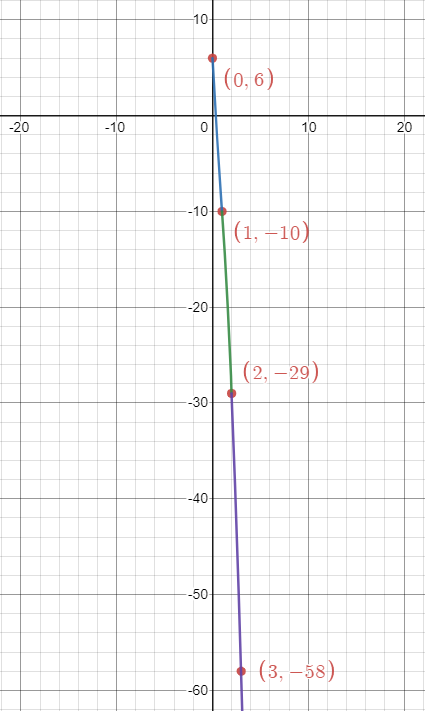
\includegraphics[scale = 1]{graphic_17.png}}
    \caption{Параболический сплайн}
\label{fig:image}
\end{figure}


\end{enumerate}

\end{document}